\clearpage
\subsection{Zebra crossing}
\label{zebrasection}
\subsubsection{Idea}
This feature will recognize a zebra crossing. The crossing is located outside the station before the blind person turns into the Sint-Denijslaan.
A zebra crossing consists of white rectangles with a certain size and shape, see Figure \ref{zebra}. However, these rectangles can be covered with dirt, making recognization difficult.
%\clearpage
\mijnfiguur{width=0.45\textwidth}{zebra}{A zebra crossing consists of white rectangles which can bo coverd with dirt}

\subsubsection{First approach}
The first approach uses a simple rectangle recognising system\footnote{This algoritm was found on github (\url{https://github.com/Itseez/opencv/blob/master/samples/cpp/squares.cpp})}.
Since the rectangle system was already used to determine the different tile sizes, the new algorithm would start from this system. With small modifications and calibrations, the program is able to find multiple rectangles. However since this approach ignores colors, found rectangles aren't always white. This created an unacceptable amount of false positives.
\npar
To solve this, the image is converted into a grayscale image. Then a small blur effect is applied to even out noise. After the noise-cancelling, the image is thresholded to create a mask. This mask is applied to the original image giving a remaining image that only has white colors, shown in Figure \ref{zebra2}.
\npar
\mijnfiguur{width=0.45\textwidth}{zebra2}{The white colors remain}
\clearpage
Since the system searches for white rectangles between a mininum and maximum size, results are improved. However false positives are still reported. To cancel out these false positives, a ratio is calculated and only rectangles whose ratio is between a lower and upper limit are allowed. This ratio enforces the shape of the rectangle while reducing false positives.
\npar
This version finds some rectangles, however if the duration of the crossing is 100 frames, only 5 frames are reported positive, this is unacceptable. Another downside is the processing time, the system that detects rectangles does mulitple iterations and searches for contours in every color dimension. This is quite useless since the image is converted to a grayscale. Then it is masked on the original image before it's handed over to the detector. Since the detector only uses one color dimension at a time, the image is again transformed. Masking and converting back and forth between colorspaces in combination with multiple iterations causes a lot of unnecessary overhead. The aforementioned problem calls for a new approach that uses less processing time and finds more white rectangles.

\subsubsection{Second approach}
The second approach will design a new findRectangle algoritm that doesn't rely on the existing one. This algoritm recieves a frame that is downsampled with the pyrDown function then upsampled with the pyrUp function to lower the noise. After that, the image is converted into a grayscale image and blurred. Then the white values are kept by thresholding the image. Once completed, the image is dilated. Both the dilation and blur effects are used to smooth the image\footnote{This is explained in a opencv tutorial found here: \url{http://docs.opencv.org/doc/tutorials/imgproc/gausian_median_blur_bilateral_filter/gausian_median_blur_bilateral_filter.html}} reducing the impact of the dirt shown in Figure \ref{zebra}. After the dilation the canny edge detection is used. Figure \ref{zebra_orig} shows the original frame while Figure \ref{zebrawitcanny} shows the edges found by the canny edge detection algorithm.
\begin{figure}[ht]
\centering
\caption{Comparison of a frame before and after the canny edge detection.}
\begin{subfigure}{.5\textwidth}
  \centering
  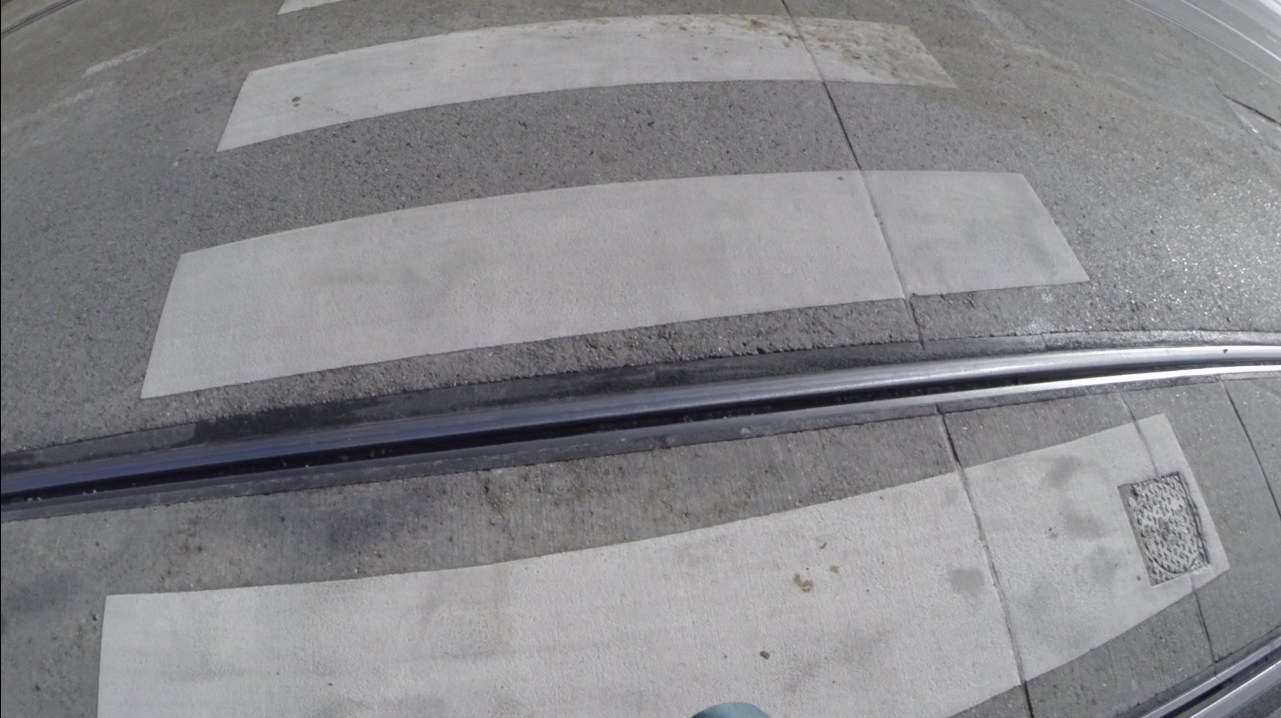
\includegraphics[width=.9\textwidth]{zebra_orig}
  \caption{Original frame\label{zebra_orig}}
\end{subfigure}%
\begin{subfigure}{.5\textwidth}
  \centering
  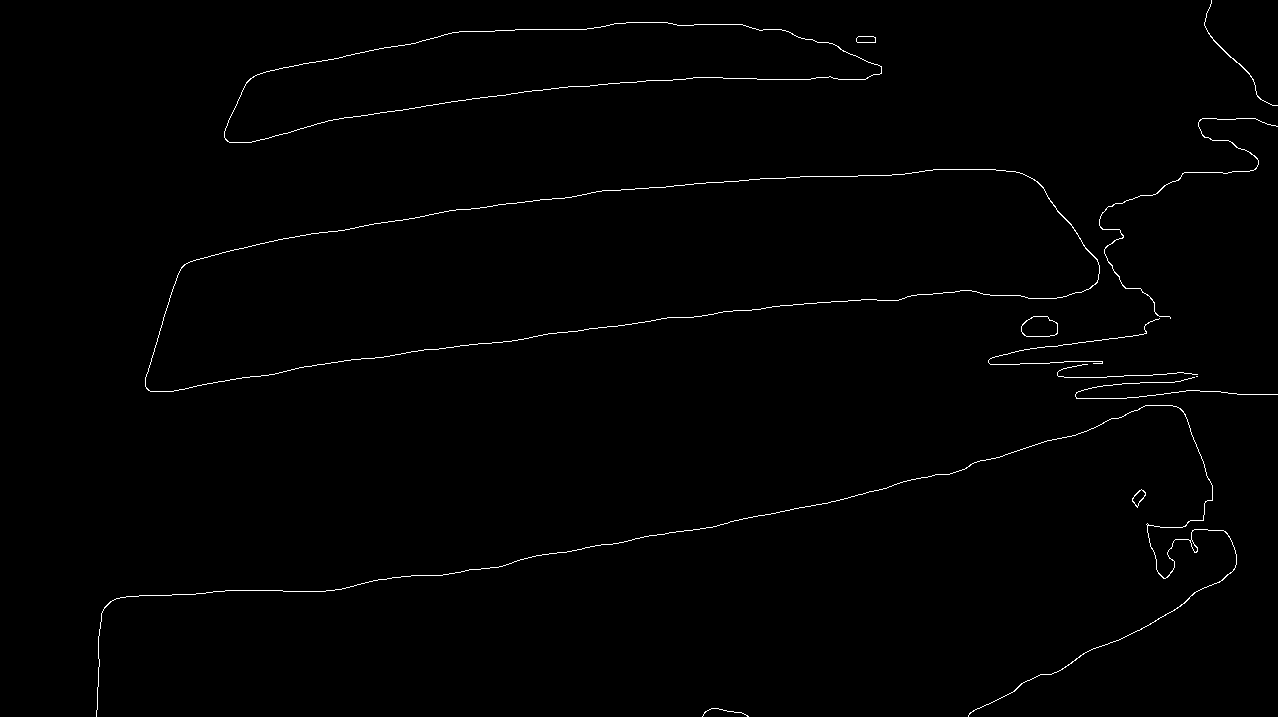
\includegraphics[width=.9\textwidth]{zebrawitcanny}
  \caption{After Canny\label{zebrawitcanny}}
\end{subfigure}
\end{figure}
\npar
Once the edges are found, the findContours function is used to find contours in the image\footnote{\url{http://docs.opencv.org/modules/imgproc/doc/structural_analysis_and_shape_descriptors.html?highlight=findcontours}}. The size and shape of each contour is tested using the ratio of the width / height.Also the size is measured. Since this function uses only one conversion and no iterations, the processing time is reduced approx to one-tenth of the original time.
\clearpage
However the second requirement of finding more rectangles isn't met. The cause of this problem is the high amount of dirt
on the white rectangles. Figure \ref{probvoor} shows the original image, Figure \ref{probna} shows the resulting canny
edge detection. It is clear that, in order to find a big rectangle in Figure \ref{probna}, the dirt must be removed. Note that not only dirt but also a shadow can cause this problem. Developping a solution for this problem takes time, so this feature isn't used for classification.
\begin{figure}[ht]
\centering
\caption{A frame showing a rectangle covered with dirt and its corresponding canny edge detection result.}
\begin{subfigure}{.5\textwidth}
  \centering
  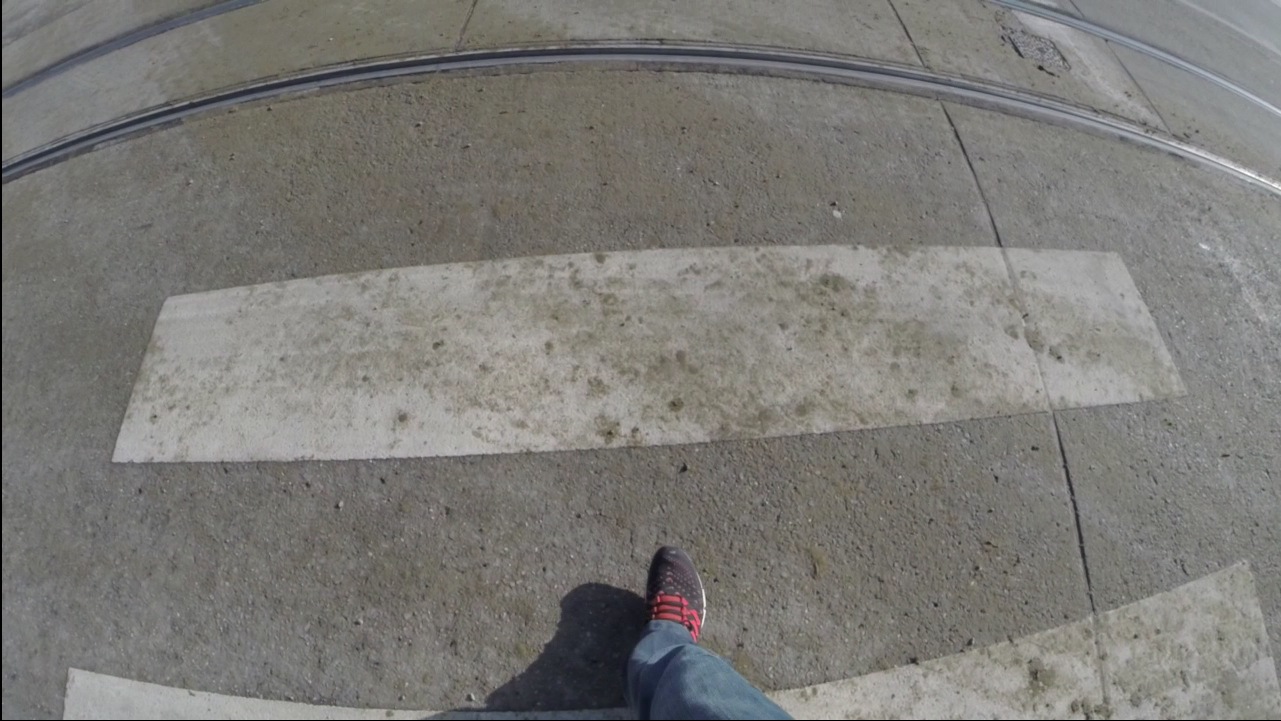
\includegraphics[width=.9\textwidth]{probvoor}
  \caption{Original frame\label{probvoor}}
\end{subfigure}%
\begin{subfigure}{.5\textwidth}
  \centering
  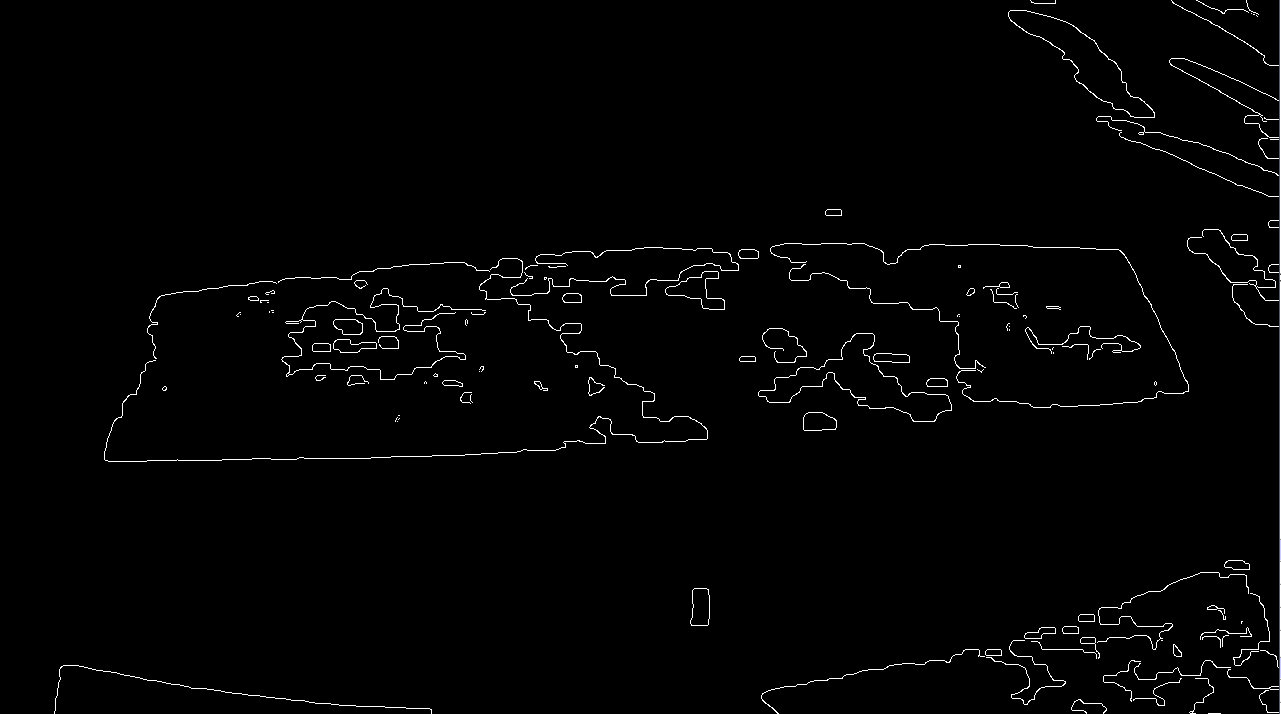
\includegraphics[width=.9\textwidth]{probna}
  \caption{\label{probna}}
\end{subfigure}
\end{figure}

\npar
When the dirt is on the edge of a rectangle, as shown in Figure \ref{dirtycorner}, the problem could be solved by ignore that edge. The edge detection won't find a rectangle but a trapezoid, shown in Figure \ref{dirtycorner2}. 
\begin{figure}[ht]
\centering
\caption{A frame showing a rectangle covered with dirt and its corresponding canny edge detection result.}
\begin{subfigure}{.5\textwidth}
  \centering
  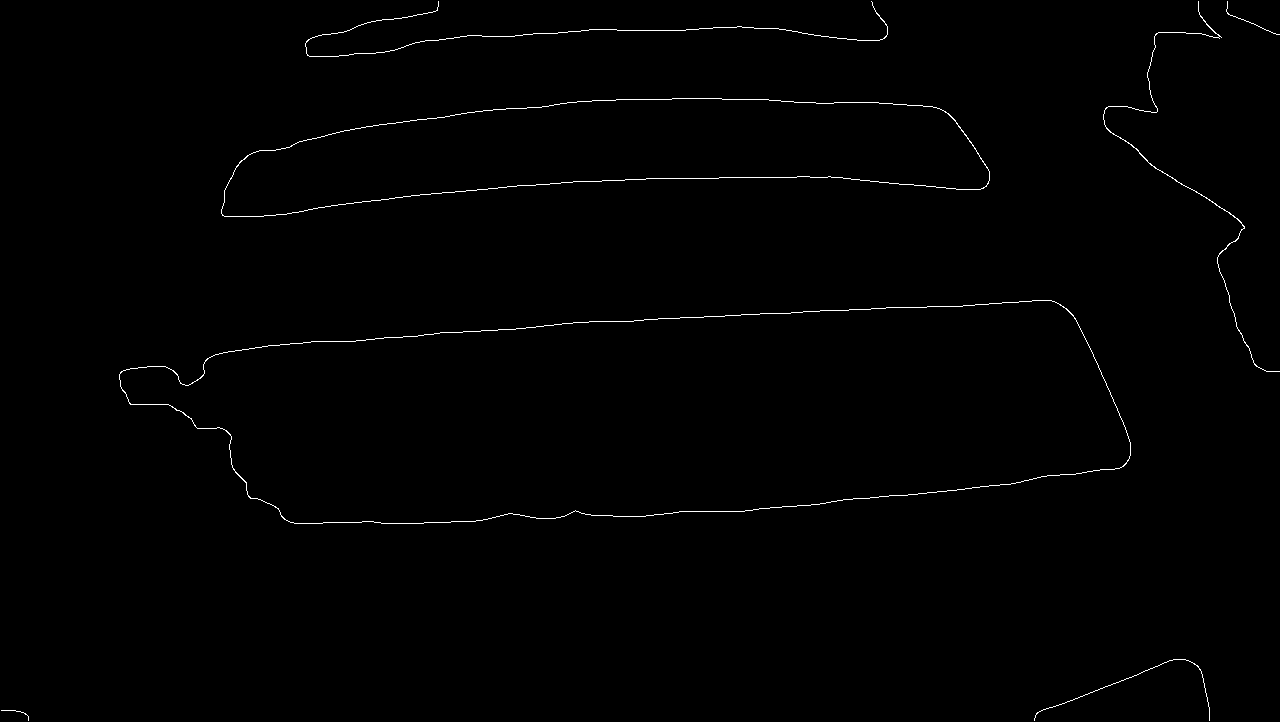
\includegraphics[width=.9\textwidth]{dirtycorner}
  \caption{Original frame\label{dirtycorner}}
\end{subfigure}%
\begin{subfigure}{.5\textwidth}
  \centering
  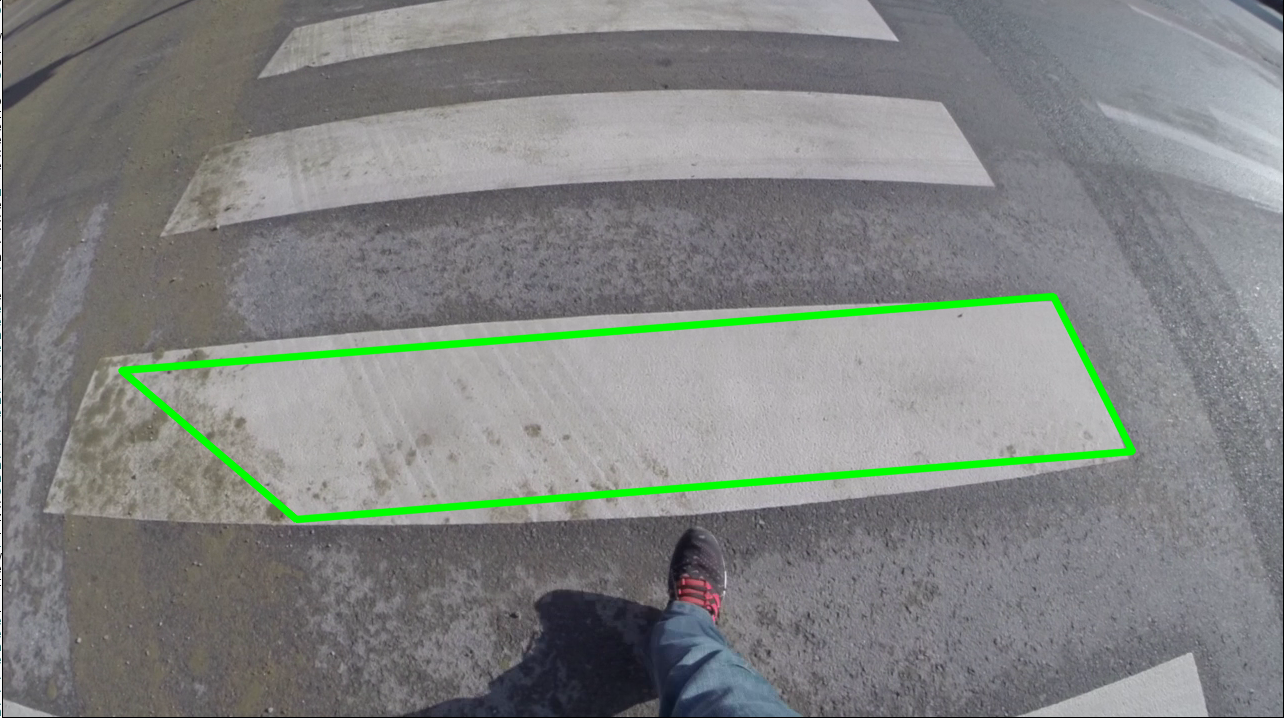
\includegraphics[width=.9\textwidth]{dirtycorner2}
  \caption{\label{dirtycorner2}}
\end{subfigure}
\end{figure}



\clearpage